% ------------------------------------------------------------------------
% bjourdoc.tex for birkjour.cls*******************************************
% ------------------------------------------------------------------------
%%%%%%%%%%%%%%%%%%%%%%%%%%%%%%%%%%%%%%%%%%%%%%%%%%%%%%%%%%%%%%%%%%%%%%%%%%

\documentclass{birkjour}

\usepackage{url}
\usepackage{commands}
%
%
% THEOREM Environments (Examples)-----------------------------------------
%
 \newtheorem{thm}{Theorem}[section]
 \newtheorem{cor}[thm]{Corollary}
 \newtheorem{lem}[thm]{Lemma}
 \newtheorem{prop}[thm]{Proposition}
 \theoremstyle{definition}
 \newtheorem{defn}[thm]{Definition}
 \theoremstyle{remark}
 \newtheorem{rem}[thm]{Remark}
 \newtheorem*{ex}{Example}
 \numberwithin{equation}{section}

\def\HOML{\entity{HOML}\xspace}
\def\HOL{\entity{HOL}\xspace}


\begin{document}

%-------------------------------------------------------------------------
% editorial commands: to be inserted by the editorial office
%
%\firstpage{1} \volume{228} \Copyrightyear{2004} \DOI{003-0001}
%
%
%\seriesextra{Just an add-on}
%\seriesextraline{This is the Concrete Title of this Book\br H.E. R and S.T.C. W, Eds.}
%
% for journals:
%
%\firstpage{1}
%\issuenumber{1}
%\Volumeandyear{1 (2004)}
%\Copyrightyear{2004}
%\DOI{003-xxxx-y}
%\Signet
%\commby{inhouse}
%\submitted{March 14, 2003}
%\received{March 16, 2000}
%\revised{June 1, 2000}
%\accepted{July 22, 2000}
%
%
%
%---------------------------------------------------------------------------
%Insert here the title, affiliations and abstract:
%


\title[Modal Collapse]
 {The Ontological Modal Collapse \\ 
 as a Collapse of the Square of Opposition}



%----------Author 1
\author[Benzm\"uller]{Christoph Benzm\"uller}

\address{%
Department of Mathematics and Computer Science\\
Arnimallee 7 \\
Room 115 \\
14195 Berlin \\
Germany
}

\email{c.benzmueller@gmail.com}

%\thanks{This work was completed with the support of ToDo}


%----------Author 3
\author[Woltzenlogel-Paleo]{Bruno Woltzenlogel Paleo}
\address{ 
Favoritenstra{\ss}e 9 \\
Room HA0402 \\
1040 Wien \\
Austria
}
\email{bruno.wp@gmail.com}




%----------classification, keywords, date
\subjclass{
Prim. 03A02;  % Philosophical aspects of logic and foundations
Sec. 68T02 % Artificial Intelligence
}

\keywords{Modal Logics, Higher-Order Logics, Ontological Argument}

\date{August 30, 2014}
%----------additions
\dedicatory{ }
%%% ----------------------------------------------------------------------

\begin{abstract}
The \emph{modal collapse} that afflicts G\"odel's modal ontological 
argument for God's existence is discussed from the perspective of the 
modal square of opposition.
\end{abstract}

%%% ----------------------------------------------------------------------
\maketitle
%%% ----------------------------------------------------------------------
%\tableofcontents
\section{Introduction}

Attempts to prove the
existence (or non-existence) of God by means of abstract, ontological
arguments are an old tradition in western philosophy, with contributions by several prominent philosophers, including St. Anselm of
Canterbury, Descartes and Leibniz. Kurt G{\"o}del studied and further improved this argument, bringing it to a mathematically more precise form, as a chain of axioms, lemmas and theorems in a modal logic \cite{GoedelNotes,ScottNotes}, shown in Fig. \ref{fig:scott}.

\begin{figure}[t]
\noindent \framebox[\columnwidth][r]{
\begin{minipage}{.94\columnwidth}\small
\begin{itemize}
\item[\textbf{A1}] Either a property or its negation is positive, but not
  both:
  $$\hol{\allq \varphi [P(\neg \varphi) \biimp \neg P(\varphi)]}$$ 
\item[\textbf{A2}] A property necessarily implied by a
  positive property is positive:
  $$\hol{\allq \varphi \allq \psi [(P(\varphi) \wedge \nec \allq x [\varphi(x)
  \imp \psi(x)]) \imp P(\psi)]}$$
\item[\textbf{T1}] Positive properties are possibly exemplified: 
  $$\hol{\allq \varphi [P(\varphi) \imp \pos \exq x \varphi(x)]}$$ 
\item[\textbf{D1}] A \emph{God-like} being possesses all positive properties: 
  $$\hol{G(x) \equiv \forall \varphi [P(\varphi) \imp \varphi(x)]}$$ 
\item[\textbf{A3}]  The property of being God-like is positive: 
  $$\hol{P(G)}$$
\item[\textbf{C\phantom{1}}] Possibly, a God-like being exists: $$\hol{\pos \exq x G(x)}$$
\item[\textbf{A4}]  Positive properties are necessarily positive: 
  $$\hol{\allq \varphi [P(\varphi) \imp \Box \; P(\varphi)]}$$ 
\item[\textbf{D2}] An \emph{essence} of an individual is a property possessed by it and necessarily implying any of its properties: $$\hol{\ess{\varphi}{x} \equiv \varphi(x) \wedge \allq
  \psi (\psi(x) \imp \nec \allq y (\varphi(y) \imp \psi(y)))}$$ 
\item[\textbf{T2}]  Being God-like is an essence of any
  God-like being: $$\hol{\allq x [G(x) \imp \ess{G}{x}]}$$
\item[\textbf{D3}] \emph{Necessary existence} of an individual is the necessary exemplification of all its essences: 
  $$\hol{\NE(x) \equiv \allq \varphi [\ess{\varphi}{x} \imp \nec
  \exq y \varphi(y)]}$$
\item[\textbf{A5}] Necessary existence is a positive property: $$\hol{P(\NE)}$$ 
\item[\textbf{L1}] If a god-like being exists, then necessarily a god-like being exists: 
  $$\hol{\exq x G(x) \imp \nec \exq y G(y)}$$
\item[\textbf{L2}] If possibly a god-like being exists, then necessarily a god-like being exists: 
  $$\hol{\pos \exq x G(x) \imp \nec \exq y G(y)} $$
%
\item[\textbf{T3}] Necessarily, a God-like being exists: $$\hol{\nec \exq x G(x)}$$ 
\end{itemize}
\end{minipage}
} \vskip-.5em
\caption{Scott's version of G\"odel's ontological argument \cite{ScottNotes}.\label{fig:scott}} 
\end{figure}


% Ontological arguments, for or against the existence of God,
% illustrate well an essential aspect of metaphysics: some (necessary) facts
% for our existing world are deduced by purely a priori, analytical means from some
% abstract definitions and axioms. % Contingent truths are to be
% distinguished from necessary truths.


G\"{o}del defines God as a being who possesses all \emph{positive}
properties and states a few reasonable (but debatable) axioms
that such properties should satisfy.  
The overall idea of G{\"o}del's proof is in the tradition of Anselm's
argument, who defined God as some entity of which nothing greater can be
conceived. Anselm argued that existence in the actual world would
make such an assumed being even greater; hence, by definition, God must
exist. However, for Anselm existence was treated as a predicate and the possibility of God's existence was assumed as granted. These issues were criticized by Kant and Leibniz, respectively, and succesfully addressed by G\"odel. 

Nevertheless, G{\"o}del's work
still leaves room for criticism. In particular, his axioms are so
strong that they entail a \emph{modal collapse} 
\cite{ToDo:sobel1987?,sobel2004logic}: 
everything that is the case is so necessarily. 
There has been an impressive body of recent and ongoing
work (cf.~\cite{sobel2004logic,Fitting,anderson90:_some_emend_of_goedel_ontol_proof,AndersonGettings,ToDo:FrodeAndHajek,ContemporaryBibliography} and the references therein)
proposing solutions for the modal collapse. 
The goal of this short note is to discuss the modal collapse from the point of view of the modal square of opposition.


\section{A Collapse of the Modal Square}

A crucial step of most ontological arguments is the claim that 
if God's existence is possible, then it is necessary. 
This is Lemma \textbf{L2} in G\"odel's proof. 
In the modal square of opposition (Fig. \ref{fig:square}), 
this is an unusual situation in which the \textbf{I} corner 
must imply and entail the \textbf{A} corner, 
in the particular case when $\phi$ is $\exq x G(x)$. 
G\"odel's proof shows that his axioms are strong enough 
to invert the direction of entailment for the sentence at issue. 
The question, however, is whether the axioms are not too strong, 
also allowing the inverted entailment for arbitrary $\phi$. 
That is essentially the question asked by Sobel \cite{Sobel1987}; 
and his proof of the modal collapse (\textbf{MC}) provides an affirmative 
answer. It is possible to show that this form of the modal 
collapse entails (in modal logic \textbf{\emph{K}}) a collapse of the modal 
square (\textbf{MC'}), causing the subcontraries to entail (and even imply) their respective contraries. Normally, as shown in Fig. \ref{fig:square}, in the modal square of opposition only the other direction of entailment holds: the contraries entail their subcontraries, assuming the \emph{modal existential import} \textbf{ExImp}.

Moreover, in any modal logic where the 
axiom \textbf{T} holds (i.e. where the accessibility relation is reflexive), a total collapse of the modalities (\textbf{MC''}) occurs. Interestingly, under this stronger form of modal collapse, the contraries entail their subcontraries even without the existential import.

\begin{figure}[t]
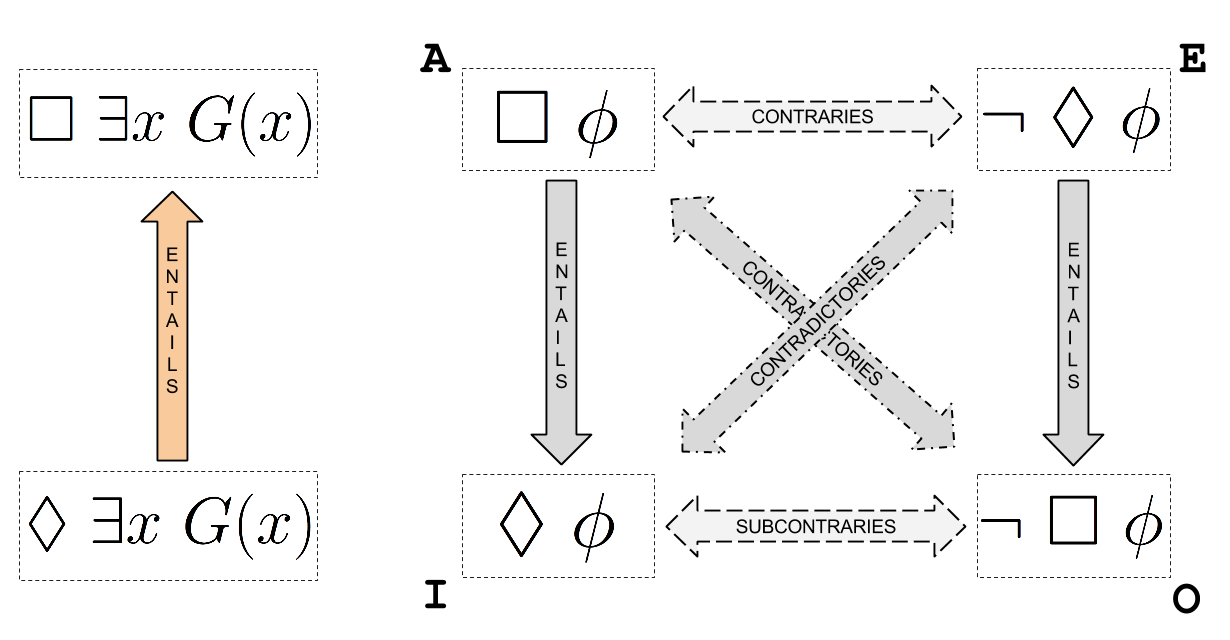
\includegraphics[width=0.9\textwidth]{./SquarePics/ModalSquare.png}
\caption{Modal Square of Opposition.}
\label{fig:square}
\end{figure}



\begin{figure}[t]
\noindent \framebox[\columnwidth][r]{
\begin{minipage}{.94\columnwidth}\small
\begin{itemize}
\item[\textbf{MC}] Everything that is the case is so necessarily:
  $\hol{\allq \phi [\phi \imp \nec \phi]}$ \\
\item[\textbf{MC'}] Everything that is possible is necessary:
  $\hol{\allq \phi [\pos \phi \imp \nec \phi]}$  \\
\item[\textbf{T}] Everything that is necessary is the case:
  $\hol{\allq \phi [\nec \phi \imp \phi]}$ \\
\item[\textbf{ExImp}] (Modal Existential Import):
  $\hol{\pos \top}$ \\
\item[\textbf{AI}] Everything that is necessary is possible:
  $\hol{\allq \phi [\nec \phi \imp \pos \phi]}$ \\
\item[\textbf{MC''}] Modalities collapse completely:
  $\hol{\allq \phi [\phi \biimp \pos \phi \biimp \nec \phi]}$
\end{itemize}
\end{minipage}
} \vskip-.5em
\caption{Modal Collapse}
\label{fig:collapse} 
\end{figure}

\newcommand{\collapse}[1]{\mathit{collapse}(#1)}

Although G\"odel's axioms lead to modal collapse, 
there are several variants (e.g. \cite{anderson,bjordal}) 
that are known to be immune to the modal collapse. 
This means there must be at least one proposition $\phi$ 
such that $\phi \imp \nec \phi$ 
(from now on abbreviated $\collapse{\phi}$) is not valid 
under the axioms and definitions used by the variant. 
But if the variant is sufficiently similar to G\"odel's argument, 
following the path deriving Lemmas \textbf{L1} and 
\textbf{L2}, then 
$\collapse{\exq x G(x)}$ must be valid. 
Therefore, one may wonder how strong is their immunity to 
the modal collapse: is there any other proposition $\phi$ 
for which $\collapse{\phi}$ is also valid?

For Anderson's emendation \cite{anderson}, for example, a form of the modal collapse (\textbf{A:MC}), restricted to positive properties applied to god-like beings, can be derived. The proof, under the modal logic \textbf{\emph{K}}, depends only on Anderson's alternative definition of god-like being (\textbf{A:D1}). This class of propositions for which the collapse occurs is tight: weaker restrictions (\textbf{A:MC1} and \textbf{A:MC2}), which could lead to larger classes, are counter-satisfiable.

\begin{figure}[t]
\noindent \framebox[\columnwidth][r]{
\begin{minipage}{.94\columnwidth}\small
\begin{itemize}
% \item[A:A1] If a property is positive, its negation is not positive:
%   $$\hol{\allq \varphi [P(\varphi) \imp \neg P(\neg \varphi)]}$$ 
% \item[A2] A property necessarily implied by a
%   positive property is positive:
%   $$\hol{\allq \varphi \allq \psi [(P(\varphi) \wedge \nec \allq x [\varphi(x)
%   \imp \psi(x)]) \imp P(\psi)]}$$
% \item[T1] Positive properties are possibly exemplified: 
%   $$\hol{\allq \varphi [P(\varphi) \imp \pos \exq x \varphi(x)]}$$ 
\item[\textbf{A:D1}] A \emph{God-like} being necessarily possesses those and only those properties that are positive: 
  $$\hol{G_A(x) \equiv \forall \varphi [P(\varphi) \biimp \nec \varphi(x)]}$$ 
\item[\textbf{A:MC}] The modal collapse happens for any positive properties applied to any god-like being:
  $$
  \hol{\allq \varphi \allq x [(P(\varphi) \wedge G_A(x)) \imp \collapse{\varphi(x)}]}
  $$
\item[\textbf{A:MC1}] The modal collapse does \emph{not} happen for positive properties applied to arbitrary individuals (\emph{counter-satisfiable}):
  $$
  \hol{\allq \varphi \allq x [P(\varphi) \imp \collapse{\varphi(x)}]}
  $$
\item[\textbf{A:MC2}] The modal collapse does \emph{not} happen for an arbitrary properties applied to a god-like being (\emph{counter-satisfiable}):
  $$
  \hol{\allq \varphi \allq x [G_A(x) \imp \collapse{\varphi(x)}]}
  $$
% \item[A3']  The property of being God-like is positive: 
%   $$\hol{P(G_A)}$$
% \item[C\phantom{1}] Possibly, a God-like being exists: $$\hol{\pos \exq x G(x)}$$
% \item[A4]  Positive properties are necessarily positive: 
%   $$\hol{\allq \varphi [P(\varphi) \imp \Box \; P(\varphi)]}$$ 
% \item[A:D2] An \emph{essence} of an individual is a property that necessarily implies those and only those properties that the individual has necessarily: $$\hol{\essA{\varphi}{x} \equiv \allq
%   \psi [\nec \psi(x) \biimp \nec \allq y (\varphi(y) \imp \psi(y))]}$$ 
% \item[T2']  Being God-like is an essence of any
%   God-like being: $$\hol{\allq x [G_A(x) \imp \essA{G_A}{x}]}$$
% \item[D3'] \emph{Necessary existence} of an individual is the necessary exemplification of all its essences: 
%   $$\hol{\NE_A(x) \equiv \allq \varphi [\essA{\varphi}{x} \imp \nec
%   \exq y \varphi(y)]}$$
% \item[A5'] Necessary existence is a positive property: $$\hol{P(\NE_A)}$$ 
% \item[L1'] If a god-like being exists, then necessarily a god-like being exists: 
%   $$\hol{\exq x G_A(x) \imp \nec \exq y G_A(y)}$$
% \item[L2'] If possibly a god-like being exists, then necessarily a god-like being exists: 
%   $$\hol{\pos \exq x G_A(x) \imp \nec \exq y G_A(y)} $$
% %
% \item[T3'] Necessarily, a God-like being exists: $$\hol{\nec \exq x G_A(x)}$$ 
\end{itemize}
\end{minipage}
} \vskip-.5em
\caption{Restricted Collapse for Anderson's Emendation \cite{ToDo:Anderson}}
\label{fig:anderson}
\end{figure}


ToDo: write a similar paragraph about Bjordal's alternative??


Independently of the variant of the ontological argument under consideration, the following can be said about the class of collapsing propositions:
\begin{enumerate}
\item Valid propositions are collapsing: if $\phi$ is valid, then $\collapse{\phi}$ is valid.
%
\item The class of collapsing propositions is closed under logical equivalence: if $\collapse{\phi}$ is valid and $\phi \biimp \phi'$ is valid, then $\collapse{\phi'}$ is valid.
%
\item The class of collapsing propositions is not generally closed under equi-validity: even if $\collapse{\phi}$ is valid and $\phi$ and $\phi'$ are equi-valid, $\collapse{\phi'}$ may not be valid.
%
\item The class of collapsing propositions is not generally closed under implication: even if $\collapse{\phi}$ is valid and $\phi \imp \phi'$ is valid, $\collapse{\phi'}$ may not be valid.
\end{enumerate}


\clearpage



\section{Final Remarks}

All results announced in this note have been obtained experimentally\footnote{The source code of the experiments are available in \url{https://github.com/FormalTheology/GoedelGod/tree/master/Formalizations/Isabelle}.} using interactive and automated theorem provers and model finders \cite{ToDo:leo,sattalax,isabelle,coq,nitpick}. 


Various slightly different versions of
axioms and definitions have been considered by G\"{o}del and by
several philosophers who commented on his proof
(cf.~\cite{sobel2004logic,anderson90:_some_emend_of_goedel_ontol_proof,AndersonGettings,Fitting,Adams,ContemporaryBibliography}).



In theoretical philosophy, formal logical confrontations with such
ontological arguments had been so far (mainly) limited to paper
and pen.  Up to now, the use of computers was prevented, because the
logics of the available theorem proving systems were not expressive
enough to formalize the abstract concepts adequately. G{\"o}del's proof
uses, for example, a complex higher-order modal logic (\HOML) to handle
concepts such as \emph{possibility} and \emph{necessity} and to support
quantification over individuals and properties.

controversies, care with parameters

ToDo: Leibniz calculemus, Rushby, Zalta \cite{oppenheimera11,rushby13}

The technique enabling this analysis is the embedding of quantified modal logics into higher-order logics \cite{J23,B9,C36}, for which automated theorem provers exist . This technique has already been succesfully employed in the verification and reconstruction of G\"odel's proof \cite{todo:all our previous papers}, and a detailed mathematical description of the technique is available in \cite{todo:ECAI}.


% \begin{defn}
% This serves as environment for definitions. Note that the text
% appears not in italics.
% \end{defn}

% \begin{equation}\label{testequation}
% \text{This is a sample equation: } c^2=a^2+b^2
% \end{equation}

% \begin{thm}[Main Theorem]
% In contrast to definitions, theorems appear typeset in italics as
% it has become more or less standard in most textbooks and
% monographs. Equations can be cited using the \verb+\eqref+ command which
% automatically adds brackets: \verb+\eqref{testequation}+ results in \eqref{testequation}.
% \end{thm}

% \begin{proof}
% A special environment is predefined: the \textit{proof} environment. Please use
% \begin{verbatim}\begin{proof}\end{verbatim}
% proof of the statement
% \begin{verbatim}\end{proof}\end{verbatim}
% for typesetting your proofs. The end-of-proof symbol $\Box$ will be added automatically.
% \end{proof}

% There are two known problems with the placement of the end-of-proof sign:

% \begin{enumerate}
%   \item if your proof ends with a\ \ s i n g l e\ \ displayed line, the end-of-proof sign would
% be placed in the line below; if you want to avoid this, write your line in the form
% \begin{verbatim}$$displayed math line \eqno\qedhere$$\end{verbatim}
% which results in

% \begin{proof}
% $$displayed math line \eqno\qedhere$$
% \end{proof}
% \item if your proof ends with an aligned displayed environment, the command
% \verb+\tag*{\qed}+ can be used to place the end-of-proof sign properly:
% \begin{verbatim}
% \begin{align*}
% \alpha&=\beta+\gamma\\
% &=\delta+\epsilon\tag*{\qed}
% \end{align*}
% \end{verbatim}
% results in
% \begin{align*}
% \alpha&=\beta+\gamma\\
% &=\delta+\epsilon\tag*{\qed}
% \end{align*}
% \end{enumerate}
% Please try to avoid using the obsolete \verb+\eqnarray+ environment. This environment has several bugs
% and has been replaced by the more flexible \AmS\ environments \verb+align, split, multline+.


% \begin{rem}
% Additional comments are being typeset without boldfaced entrance
% word as they may be minor important.
% \end{rem}

% \begin{ex}
% For some constructs, even no number is required.
% \end{ex}

% Displayed equations may be numbered like the following one:
% \begin{equation}
% \sqrt{1-\sin^2(x)}=|\cos(x)|.
% \end{equation}



% ------------------------------------------------------------------------

% \subsection*{Acknowledgment}
% Many thanks to ...

\begin{thebibliography}{1}

\bibitem{Adams}
R.M. Adams, `Introductory note to *1970', in {\em {Kurt G\"odel: Collected
  Works Vol. 3: Unpubl. Essays and Letters}}, Oxford Univ. Press, (1995).

\bibitem{AndersonGettings}
A.C. Anderson and M.~Gettings, `G\"odel ontological proof revisited', in {\em
  {G\"odel'96: Logical Foundations of Mathematics, Computer Science, and
  Physics: Lecture Notes in Logic 6}},  167--172, {Springer}, (1996).

\bibitem{anderson90:_some_emend_of_goedel_ontol_proof}
C.A. Anderson, `Some emendations of {G{\"o}del's} ontological proof', {\em
  Faith and Philosophy}, {\bf 7}(3), (1990).

\bibitem{Andrews:gmae72}
P.B. Andrews, `General models and extensionality', {\em Journal of Symbolic
  Logic}, {\bf 37}(2),  395--397, (1972).

\bibitem{andrewsSEP}
P.B. Andrews, `Church's type theory', in {\em The Stanford Encyclopedia of
  Philosophy}, ed., E.N. Zalta, spring 2014 edn., (2014).

\bibitem{C36}
C.~Benzm{\"u}ller, `{HOL} based universal reasoning', in {\em Handbook of the
  4th World Congress and School on Universal Logic}, ed., J.Y. Beziau~et al.,
  pp. 232--233, Rio de Janeiro, Brazil, (2013).

\bibitem{B5}
C.~Benzm{\"u}ller and D.~Miller, `Automation of higher-order logic', in {\em
  Handbook of the History of Logic, Volume 9 --- Logic and Computation},
  Elsevier, (2014).
\newblock Forthcoming; preliminary version available at
  {http://christoph-benzmueller.de/papers/B5.pdf}.

\bibitem{C34}
C.~Benzm{\"u}ller, J.~Otten, and Th. Raths, `Implementing and evaluating
  provers for first-order modal logics', in {\em Proc. of the 20th European
  Conference on Artificial Intelligence (ECAI)}, pp. 163--168, (2012).

\bibitem{B9}
C.~Benzm{\"u}ller and L.C. Paulson, `Exploring properties of normal multimodal
  logics in simple type theory with {LEO-II}', in {\em {Festschrift in Honor of
  {Peter B. Andrews} on His 70th Birthday}}, ed., C.~Benzm{\"u}ller~et al.,
  386--406, College Publications, (2008).

\bibitem{J23}
C.~Benzm{\"u}ller and L.C. Paulson, `Quantified multimodal logics in simple
  type theory', {\em Logica Universalis}, {\bf 7}(1),  7--20, (2013).

\bibitem{LEO-II}
C.~Benzm{\"u}ller, F.~Theiss, L.~Paulson, and A.~Fietzke, `{LEO-II} - a
  cooperative automatic theorem prover for higher-order logic', in {\em
  Proc.~of IJCAR 2008}, number 5195 in LNAI, pp. 162--170. Springer, (2008).

\bibitem{J30}
C.~Benzm{\"u}ller and B.~Woltzenlogel-Paleo, `Formalization, mechanization and
  automation of {G{\"o}del's} proof of {God's} existence', {\em
  arXiv:1308.4526}, (2013).

\bibitem{J28}
C.~Benzm\"uller and B.~Woltzenlogel-Paleo, `{G{\"o}del's God in Isabelle/HOL}',
  {\em Archive of Formal Proofs}, (2013).

\bibitem{W50}
C.~Benzm\"uller and B.~Woltzenlogel-Paleo, `G\"odel's {God} on the computer',
  in {\em Proceedings of the 10th International Workshop on the Implementation
  of Logics}, EPiC Series. EasyChair, (2013).
\newblock Invited abstract.

\bibitem{Coq}
Y.~Bertot and P.~Casteran, {\em {Interactive Theorem Proving and Program
  Development}}, Springer, 2004.

\bibitem{Nitpick}
J.C. Blanchette and T.~Nipkow, `Nitpick: A counterexample generator for
  higher-order logic based on a relational model finder', in {\em Proc. of ITP
  2010}, number 6172 in LNCS, pp. 131--146. Springer, (2010).

\bibitem{Satallax}
C.E. Brown, `Satallax: An automated higher-order prover', in {\em Proc. of
  IJCAR 2012}, number 7364 in LNAI, pp. 111 -- 117. Springer, (2012).

\bibitem{ContemporaryBibliography}
R.~Corazzon.
\newblock Contemporary~bibliography~on~ontological~arguments: {\scriptsize
  \url{http://www.ontology.co/biblio/ontological-proof-contemporary-biblio.htm}}.

\bibitem{Fitting}
M.~Fitting, {\em Types, Tableaux and G\"odel's God}, Kluwer, 2002.

\bibitem{fitting98}
M.~Fitting and R.L. Mendelsohn, {\em First-Order Modal Logic}, volume 277 of
  {\em Synthese Library}, Kluwer, 1998.

\bibitem{Gallin75}
D.~Gallin, {\em Intensional and Higher-Order Modal Logic}, North-Holland, 1975.

\bibitem{garbacz12:_prover_simpl_expal_away}
P.~Garbacz, `{PROVER9's} simplifications explained away', {\em Australasian
  Journal of Philosophy}, {\bf 90}(3),  585--592, (2012).

\bibitem{GoedelNotes}
K.~G\"odel, {\em Appx.A: Notes in Kurt G\"odel's Hand},  144--145.
\newblock In  \cite{sobel2004logic}, 2004.

\bibitem{Henkin50}
L.~Henkin, `Completeness in the theory of types', {\em Journal of Symbolic
  Logic}, {\bf 15}(2),  81--91, (1950).

\bibitem{homl}
R.~Muskens, `{Higher Order Modal Logic}', in {\em Handbook of Modal Logic},
  ed., P~Blackburn~et al.,  621--653, Elsevier, Dordrecht, (2006).

\bibitem{Isabelle}
T.~Nipkow, L.C. Paulson, and M.~Wenzel, {\em {Isabelle/HOL: A Proof Assistant
  for Higher-Order Logic}}, number 2283 in LNCS, Springer, 2002.

\bibitem{oppenheimera11}
P.E. Oppenheimer and E.N. Zalta, `A computationally-discovered simplification
  of the ontological argument', {\em Australasian Journal of Philosophy}, {\bf
  89}(2),  333--349, (2011).

\bibitem{rushby13}
J.~Rushby, `The ontological argument in {PVS}', in {\em Proc.~of CAV Workshop
  ``Fun With Formal Methods''}, St. Petersburg, Russia,, (2013).

\bibitem{Schulz:AICOM-2002}
S.~Schulz, `E -- a brainiac theorem prover', {\em {AI Communications}}, {\bf
  15}(2),  111--126, (2002).

\bibitem{ScottNotes}
D.~Scott, {\em Appx.B: Notes in Dana Scott's Hand},  145--146.
\newblock In  \cite{sobel2004logic}, 2004.

\bibitem{sobel2004logic}
J.H. Sobel, {\em Logic and Theism: Arguments for and Against Beliefs in God},
  Cambridge U. Press, 2004.

\bibitem{sutcliffe2009tptp}
G.~Sutcliffe, `The {TPTP} problem library and associated infrastructure', {\em
  Journal of Automated Reasoning}, {\bf 43}(4),  337--362, (2009).

\bibitem{J22}
G.~Sutcliffe and C.~Benzm{\"u}ller, `Automated reasoning in higher-order logic
  using the {TPTP THF} infrastructure.', {\em Journal of Formalized Reasoning},
  {\bf 3}(1),  1--27, (2010).

\bibitem{J29}
B.~Woltzenlogel-Paleo and C.~Benzm{\"u}ller, `Automated verification and
  reconstruction of {G\"odel's} proof of {God's} existence', {\em OCG J.},
  (2013).

\end{thebibliography}


% ------------------------------------------------------------------------
\end{document}
% ------------------------------------------------------------------------
